\chapter{Search for MSSM $\PH \to hh \to \Pgt\Pgt bb$}
\label{chap:Hhh}

As described in detail in section~\ref{chap:theory}, there are many popular MSSM
models which incorporate the 125 GeV Higgs. As seen in Chapter
\ref{chap:httmssm}, the $\PH \to \Pgt\Pgt$ analysis is very successful in 
setting limits on various MSSM models. The $\PH \to \Pgt \Pgt$ result primarily sets
limits on the high $\tan\beta$ regions, and so with large amounts of the
$m_{A}-\tan\beta$plane ruled out for such MSSM scenarios, focus shifts more 
to the regions which are still allowed, in particular the low $\tan\beta$.

In certain low $\tan\beta$ regions of the MSSM, the branching ratio for the
decay of the heavy neutral scalar Higgs, H, into two of the light Higgs bosons, h,
BR($\PH \to hh$), is enhanced. Thus we could consider models in which the
light Higgs has a mass of 125 GeV and is the Higgs particle discovered at the
LHC, and as such we could get production of a pair of these light Higgs from the
heavier Higgs in the MSSM. The range of heavy Higgs masses in consideration is from 260 GeV
(driven by the kinematic threshold for the producton of two 125 GeV Higgs
bosons) up to 350 GeV (above which the branching ratio for Higgs decaying into
tops becomes overwhelmingly high).

When looking for two 125 GeV Higgs bosons, the final state consisting of two
$\tau$ leptons and two b quarks has some sensitivity. Hence we can use the
inclusive selection from the $\PH \to \Pgt\Pgt$ and require additional jets
to form the $h \to bb$. In this way we can use a large amount of the
expertise and methods from chapters \ref{chap:httsm} and \ref{chap:httmssm}, 
to design a new analysis to target $\PH \to hh \to \Pgt\Pgt bb$.

\section{Event Selection}

In signal events of all $M_{H}$ hypotheses, the reconstructed $m_{bb}$ and
$m_{\tau\tau}$ will be consistent with a $125 \GeV$ $\Ph$ decay. This fact is exploited to greatly
enhance the selection of signal over background events, by cutting in window of
$70 < m_{bb} < 150~\GeV$ and $90 < m_{\tau\tau} < 150~\GeV$. 

\section{Kinematic Fitting to extract $M_{H}$}

In addition to applying cuts on $m_{bb}$ and $m_{\tau\tau}$, the condition that
both values should be consistent with $125~\GeV$ can be used further in
calculating the reconstructed $M_{H}$. This quantity can be reconstructed simply
by combining the visible taus, $\MET$ and the b-jets, denoted by $M_{\tau\tau bb}$.
A better reconstruction is obtained by using the conditions on $m_{bb}$ and
$m_{\tau\tau}$ in a kinematic fit. 

In this method, observables related to the
event kinematics are varied within the measurement uncertainties in order to
find the values which best fulfil a kinematic constraint. In this case, the
variables being varied correspond to the energies of the taus and b-jets and the
kinematic constraints are that $m_{bb} = m_{\tau\tau} = m_{h} = 125~\GeV$. Differences
between the measured value and the constraint are accounted for in a cost
function $\chi^{2}$ which is minimised in the fitting procedure.  

For the b-jets, it is assumed that the reconstructed position in terms of the
angles $\eta_{j}$ and $\phi_{j}$ is known to great accuracy, and the largest
uncertainty is in the measurement of the energy. Thus in the fit, only the
energy of the jets is varied, and the position is kept constant. To first
approximation any uncertainty in energy directly translates to an uncertainty in
momentum related by the quantity $\beta = p/E$, which is assumed to be constant and 
not varied in the fit. The energy of the first b-jet is varied, and then the
energy of the second b-jet can be related to the first using the following
kinematic conditions:

\begin{equation}
m_{H}^{2} = p_{b_{1}}^{2} + p_{b_{2}}^{2,fit} + 2p_{b_{1}}p_{b_{2}}^{fit} 
          = m_{b_{1}}^{2} + \frac{E_{b_{2}}^{2,fit}}{\gamma_{b_{2}}^{2}} + 2E_{b_{1}}E_{b_{2}}^{fit}\left(1-\beta_{b_{1}}\beta_{b_{2}}\right),   
\label{eq:bjetkinfit}         
\end{equation}

where $\gamma_{b_{1,2}} = 1/\sqrt{1-\beta_{b_{1,2}}^{2}}$. The term A is
assumed to be constant and hence can be derived from the pre-fit event
kinematics as:

\begin{equation}
A = \frac{m_{b_{1}b_{2}}^{2} - m_{b_{1}}^{2} - m_{b_{2}}^{2}}{2E_{b_{1}}E_{b_{2}}} , 
\end{equation}

which allows equation \ref{eq:bjetkinfit} to be reduced to:

\begin{equation}
E_{b_{2}}^{fit} = E_{b_{1}}A\gamma_{b_{2}}^{2}\left(-1 + \sqrt{1 +
\frac{m_{h}^{2} -
m_{b_{1}^{2}}}{\left(E_{b_{1}}A\gamma_{b_{2}}\right)^{2}}}\right) .
\label{eq:bjetrelation}
\end{equation}

A $\chi^{2}$ quantity can then be constructed to quantify how much the fit has
modified the b-jet energy as:

\begin{equation}
\chi_{b_{1,2}}^{2} = \frac{E_{b_{1,2}}^{fit} -
E_{b_{1,2}}^{meas}}{\sigma_{b_{1,2}}}
\end{equation}

where $E_{b_{1,2}}^{meas}$ is the measured b-jet energy and $\sigma_{b_{1,2}}$
is the b-jet energy resolution. The value of $\sigma_{b_{1,2}}$ is estimated
using a \ac{MC} sample in different bins of $\eta$ and $\pt$. 

The $\Pgt$s are treated in a slightly different way in the fit due to the $\MET$
associated with their decays. It is assumed that the collinear approximation
holds such that the visible products are produced in the same direction as the
original tau. This direction is assumed to be known to a high degree of
accuracy, as in the case of the b-jets, and so is not varied in the fit. Thus as
in the case of the b-jets, only the energy of one $\Pgt$ is free in the fit, and
the energy of the other $\Pgt$ can be related to the first in an analogous way
to in equation \ref{eq:bjetrelation}. The mass of either $\Pgt$ lepton is kept
constant at $m_{\Pgt}$.  

In order to find the correct $\Pgt$ energies, additional constraints are put on
the event using the $\MET$ to enforce that the heavy Higgs recoil from the fit
is close to the reconstructed recoil. The recoil from the fit can be defined as:
%check this equation - should they all be p_T?
\begin{equation}
p_{T,recoil}^{fit} = - p_{T,b_{1}}^{fit} - p_{T,b_{2}}^{fit} -
p_{T,\Pgt_{1}}^{fit} - p_{T,\Pgt_{2}}^{fit} = - p_{T,H}^{fit} ,
\end{equation}

and the measured recoil as:

\begin{equation}
p_{T,recoil}^{meas} = - p_{T,miss}^{meas} - p_{T,b_{1}}^{meas} - p_{T,b_{2}}^{meas} -
p_{T,\Pgt_{1}^{vis}}^{meas} - p_{T,\Pgt_{2}^{vis}}^{meas} = - p_{T,H}^{meas}
\end{equation}

The $\chi^{2}$ term corresponding to the agreement between these two quantities
can be constructed as:

%\begin{equation}
%\chi_{recoil}^{2} = 
%\end{equation}

The total $\chi^{2}$ to be minimised by the fit is then given by:

\begin{equation}
\chi^{2}= \chi_{b_{1}}^{2} + \chi_{b_{2}}^{2} + \chi_{recoil}^{2},
\end{equation}

which is a two dimensional function in variables $E_{b_{1}}$ and $\Pgt_{b_{1}}$.

The output of the kinematic fit is the 4-vector of each of the taus and b-jets,
with the energy and momentum corrected by the result of the fit. Figure \ref{}
shows the difference between the heavy Higgs mass as reconstructed by
$M_{\Pgt\Pgt bb}$ and from the kinematic fit, denoted $M_{H}^{kinfit}$. It can
be seen that both the mean and resolution of $M_{H}$ is greatly improved in
signal.

\section{Control Plots}

For the preselection and separation of events into categories, there are several
kinematic variables of interest. A selection of these including b-jet related
variables, kinematics of the tau candidates, $\MET$ and $m_{T}$ are shown in
Figs.~\ref{fig:resultsControlPlotsTauPairMuTau}
and~\ref{fig:resultsControlPlotsJetPairMuTau} for the $\mu\tau_{had}$ channel
, Figs.~\ref{fig:resultsControlPlotsTauPairETau} and
~\ref{fig:resultsControlPlotsJetPairETau} for the $e\tau_{had}$ channel.
These plots are made before events are split into categories, and use all events
with all least 2 jets (no additional b-tag requirements).


\begin{figure}
\begin{center}
\subfloat[]{
    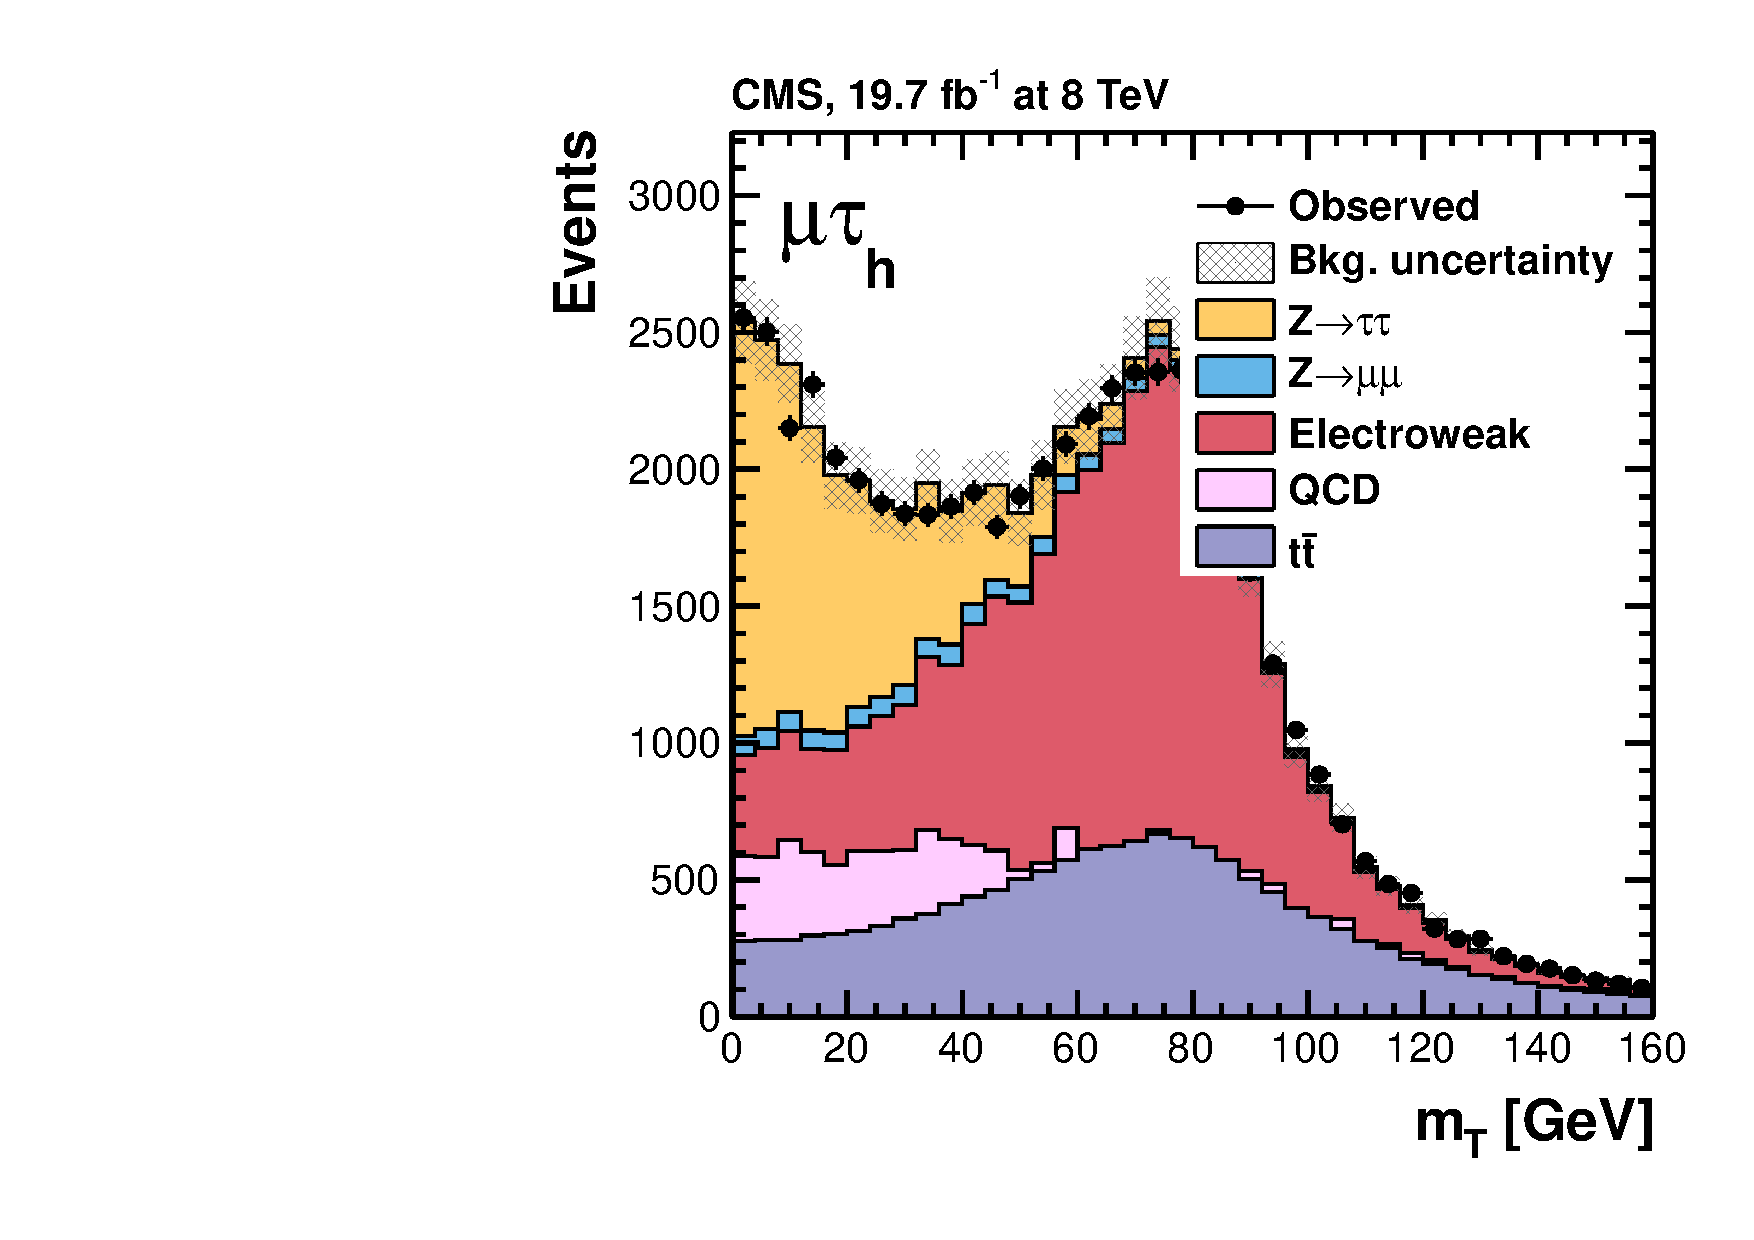
\includegraphics[width=0.4\textwidth]
      {plots/Hhh/ControlPlots/mutau/mt_1_2jetinclusive_mt_2012.pdf}}
\subfloat[]{
    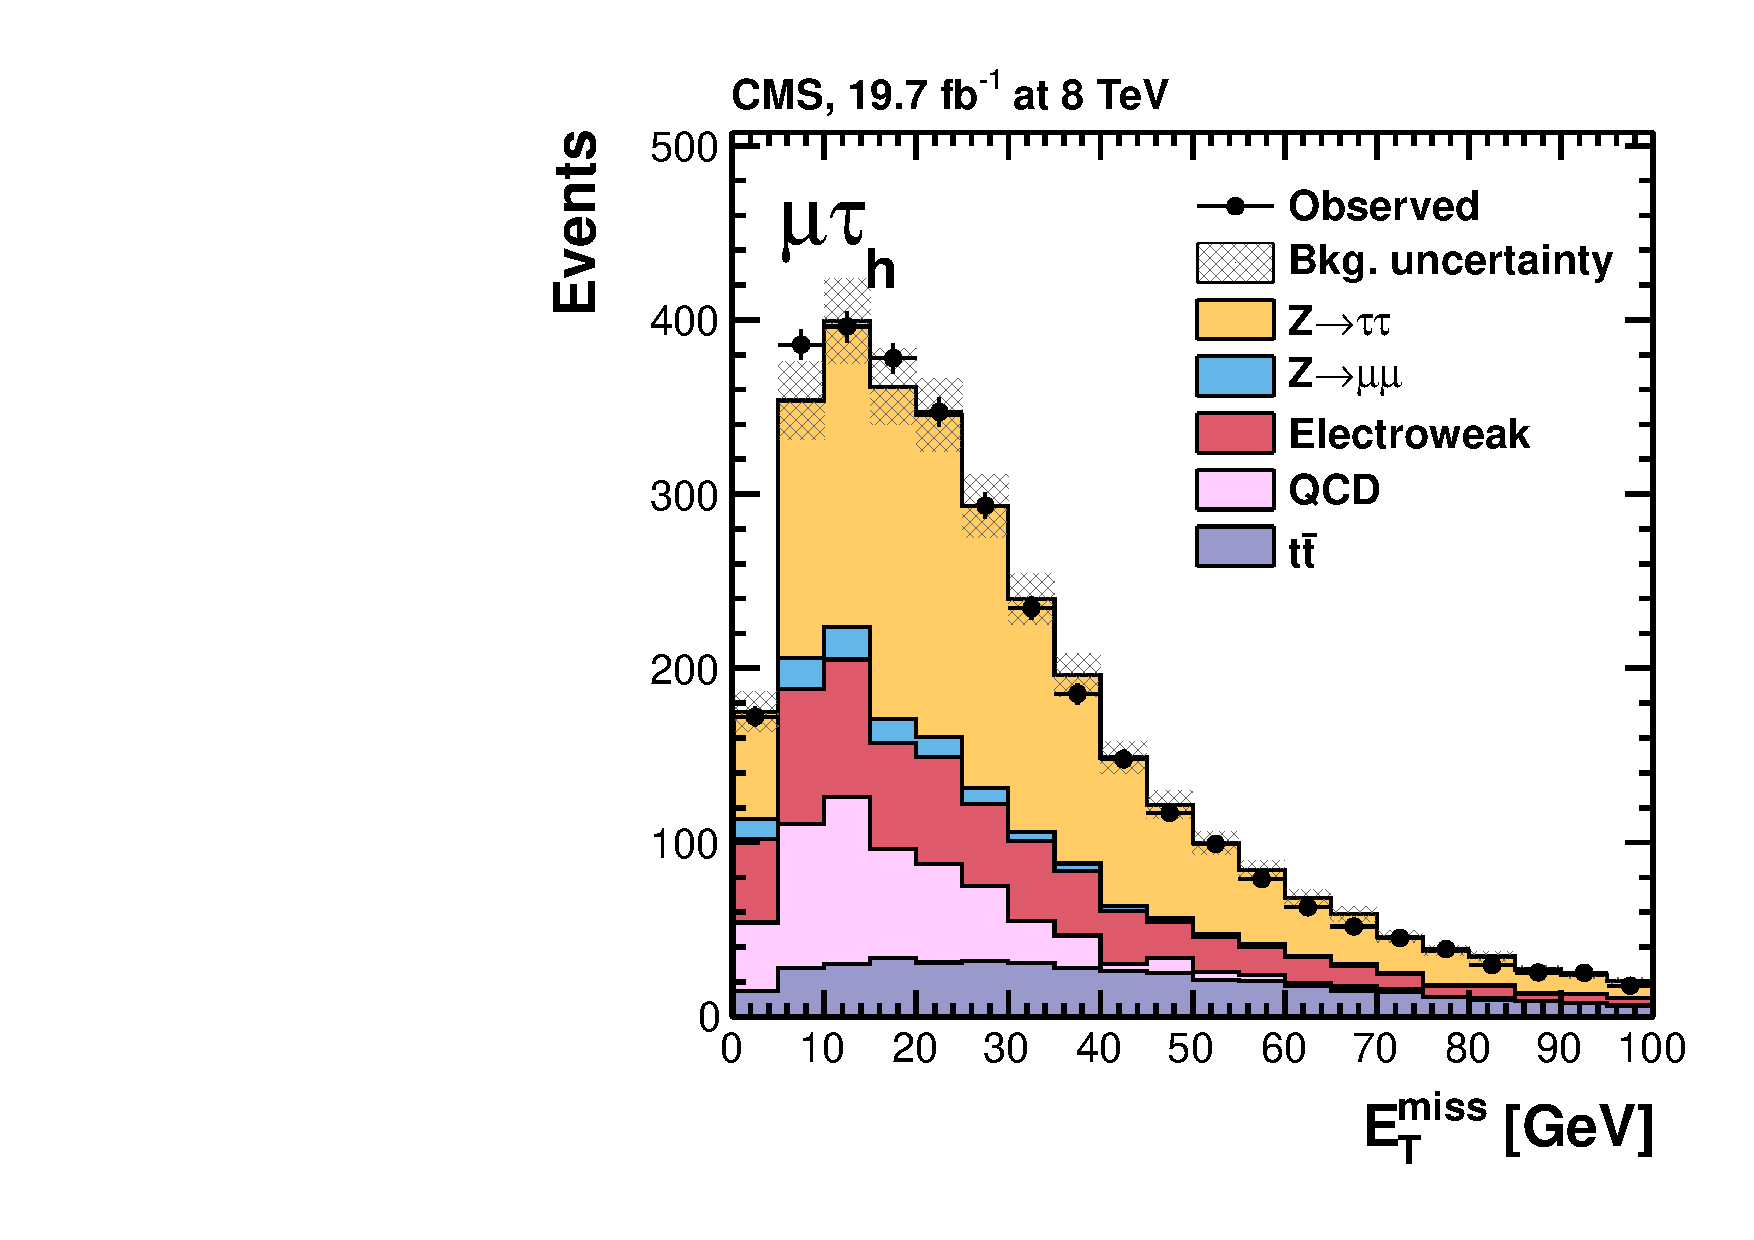
\includegraphics[width=0.4\textwidth] 
      {plots/Hhh/ControlPlots/mutau/met_2jetinclusive_mt_2012.pdf}} 

\subfloat[]{
    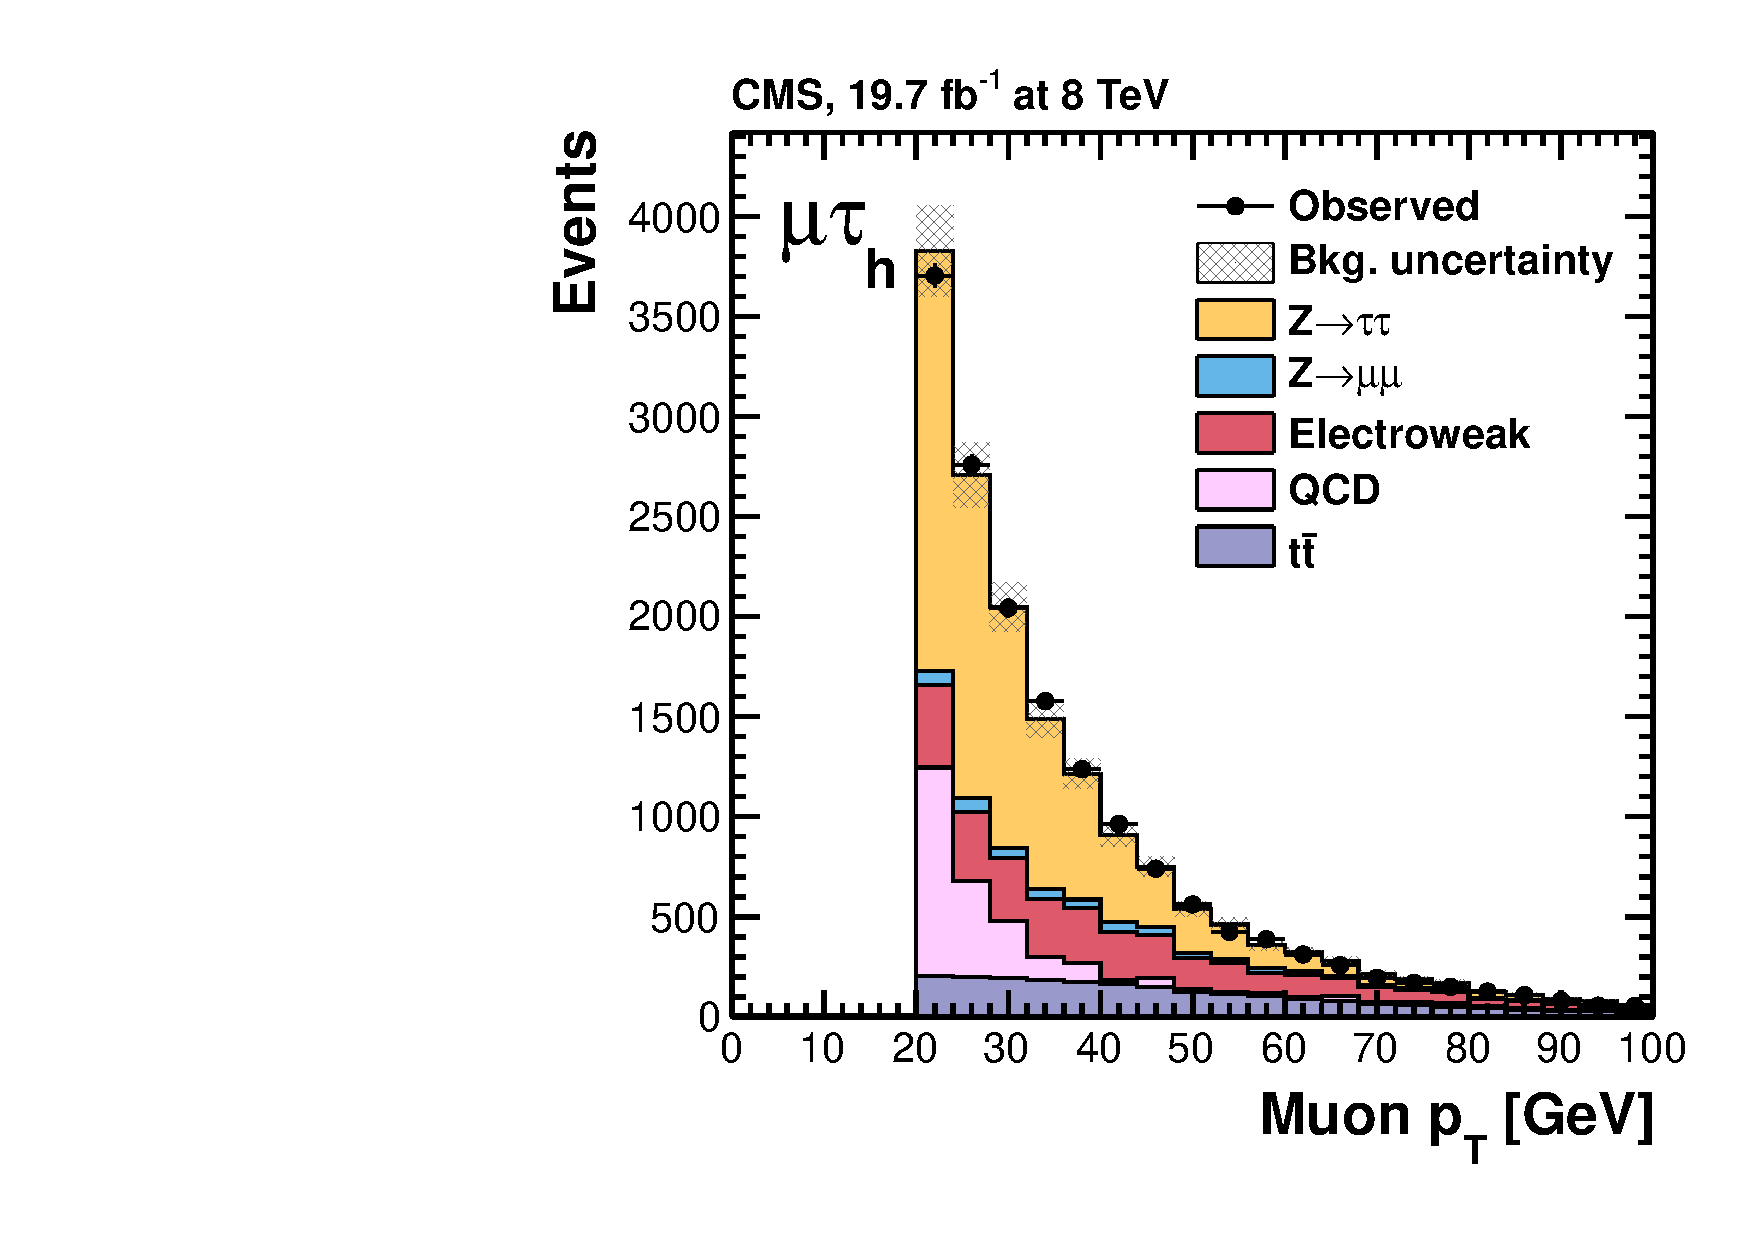
\includegraphics[width=0.4\textwidth]
      {plots/Hhh/ControlPlots/mutau/pt_1_2jetinclusive_mt_2012.pdf}}
\subfloat[]{
    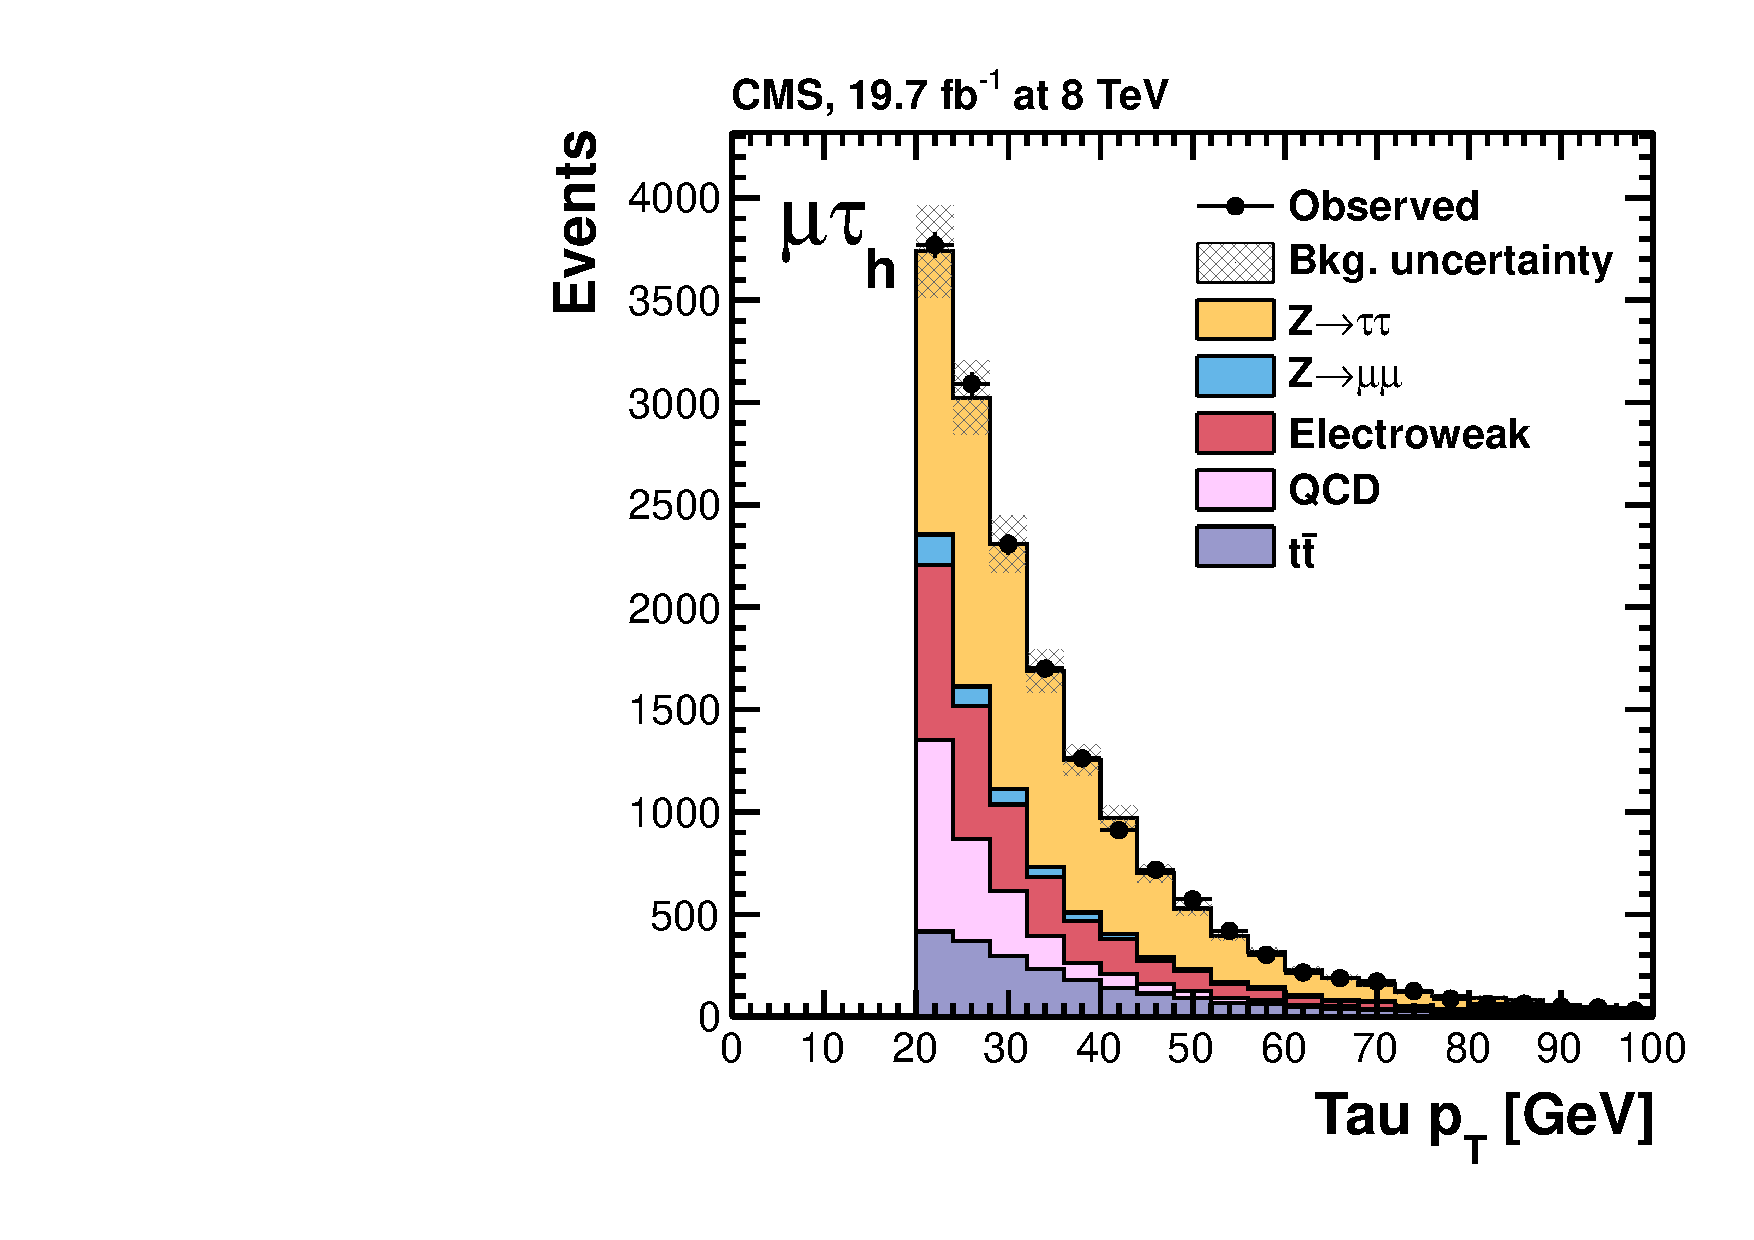
\includegraphics[width=0.4\textwidth]
      {plots/Hhh/ControlPlots/mutau/pt_2_2jetinclusive_mt_2012.pdf}} 

\subfloat[]{
    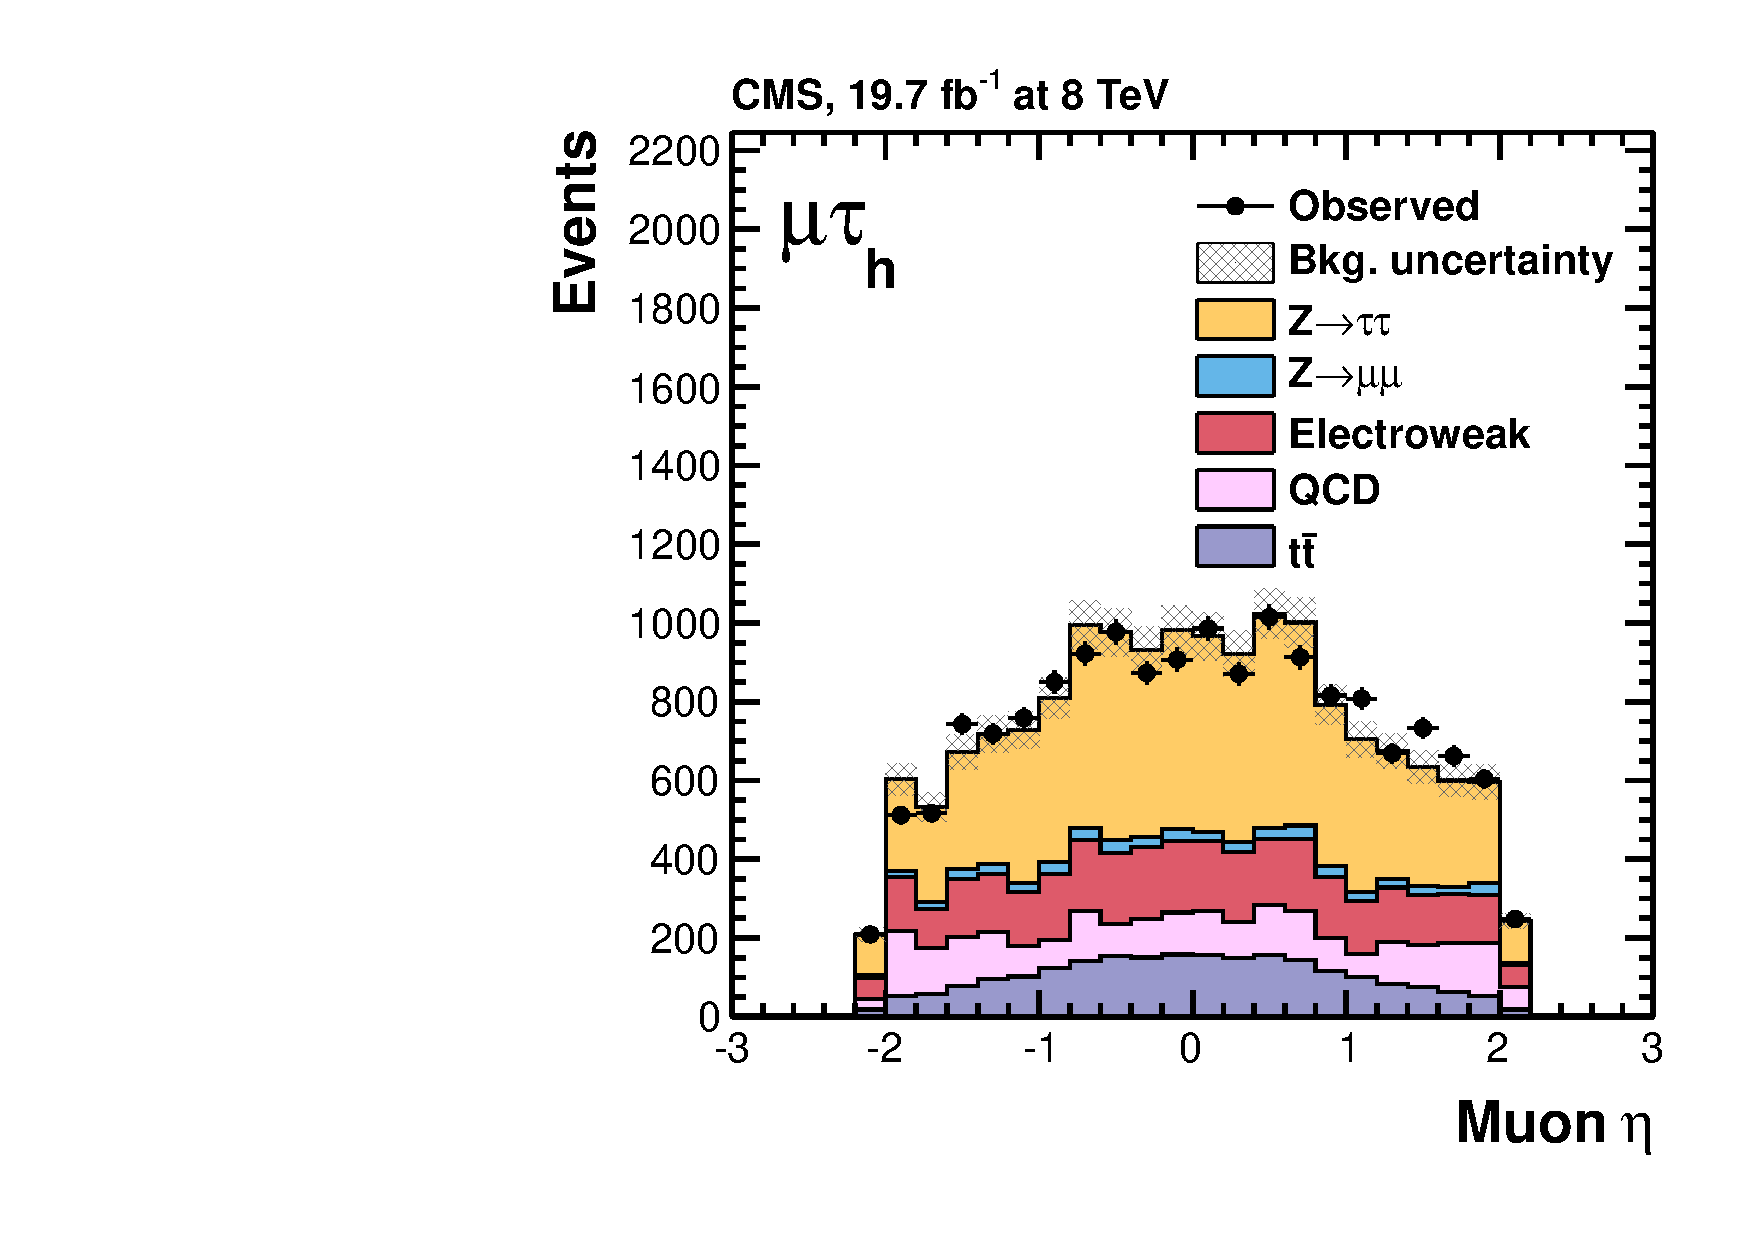
\includegraphics[width=0.4\textwidth]
      {plots/Hhh/ControlPlots/mutau/eta_1_2jetinclusive_mt_2012.pdf}}
\subfloat[]{
    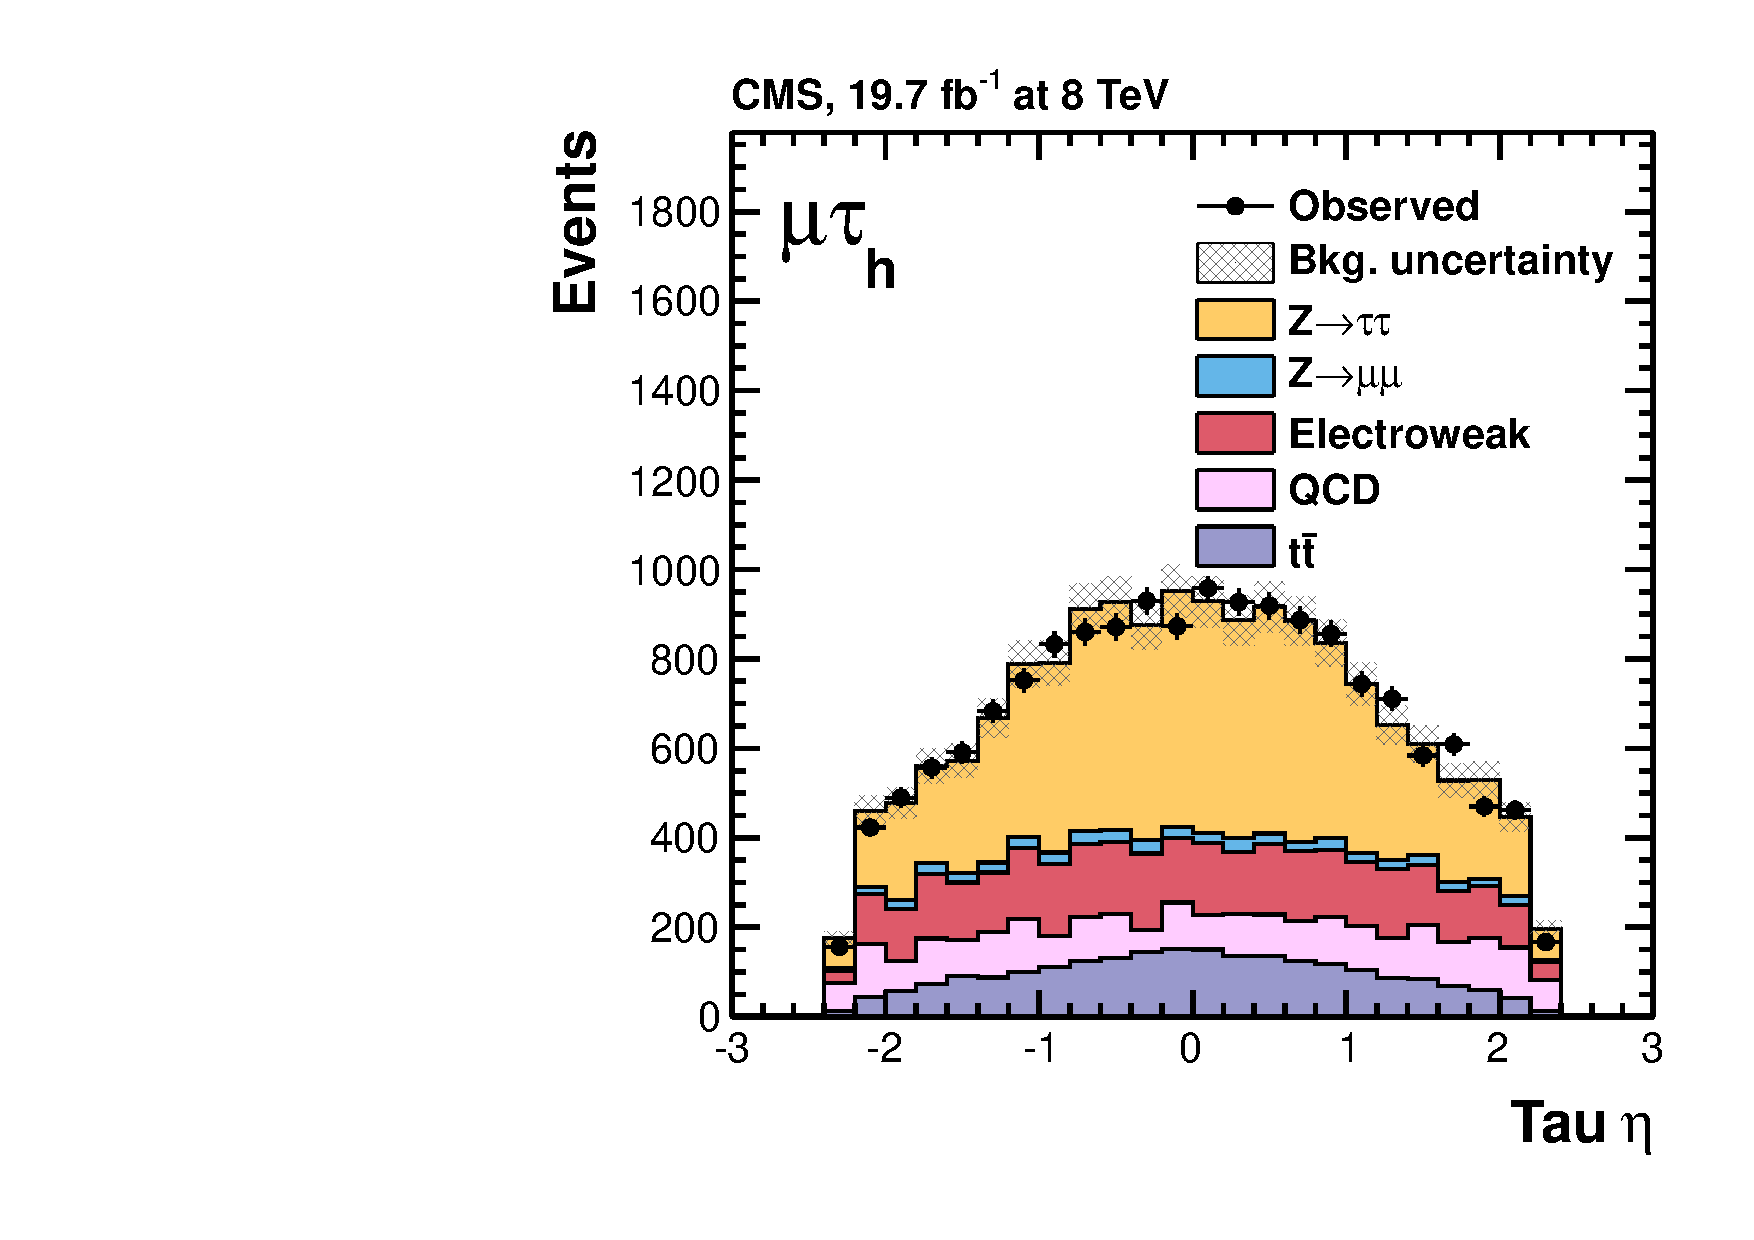
\includegraphics[width=0.4\textwidth]
      {plots/Hhh/ControlPlots/mutau/eta_2_2jetinclusive_mt_2012.pdf}}
\end{center}
\caption{
  Distributions of relevant kinematic variables for events with at least 2 jets
  in the $\mu\tau_{had}$ channel. The variable shown in a) is $m_{T}$, on which
  a cut of $m_{T} < 30$ is applied for the rest of the plots, which
  show b) $\MET$, c) $\pt$ of the muon, d) $\pt$ of the tau, e) $\eta$ of the
  muon and f) $\eta$ of the tau. 
  Expected background contributions are shown for the values of nuisance parameters
  obtained by fitting the signal plus background hypothesis to the data.
}
\label{fig:resultsControlPlotsTauPairMuTau}
\end{figure} 

\begin{figure}
\begin{center}
\subfloat[]{
    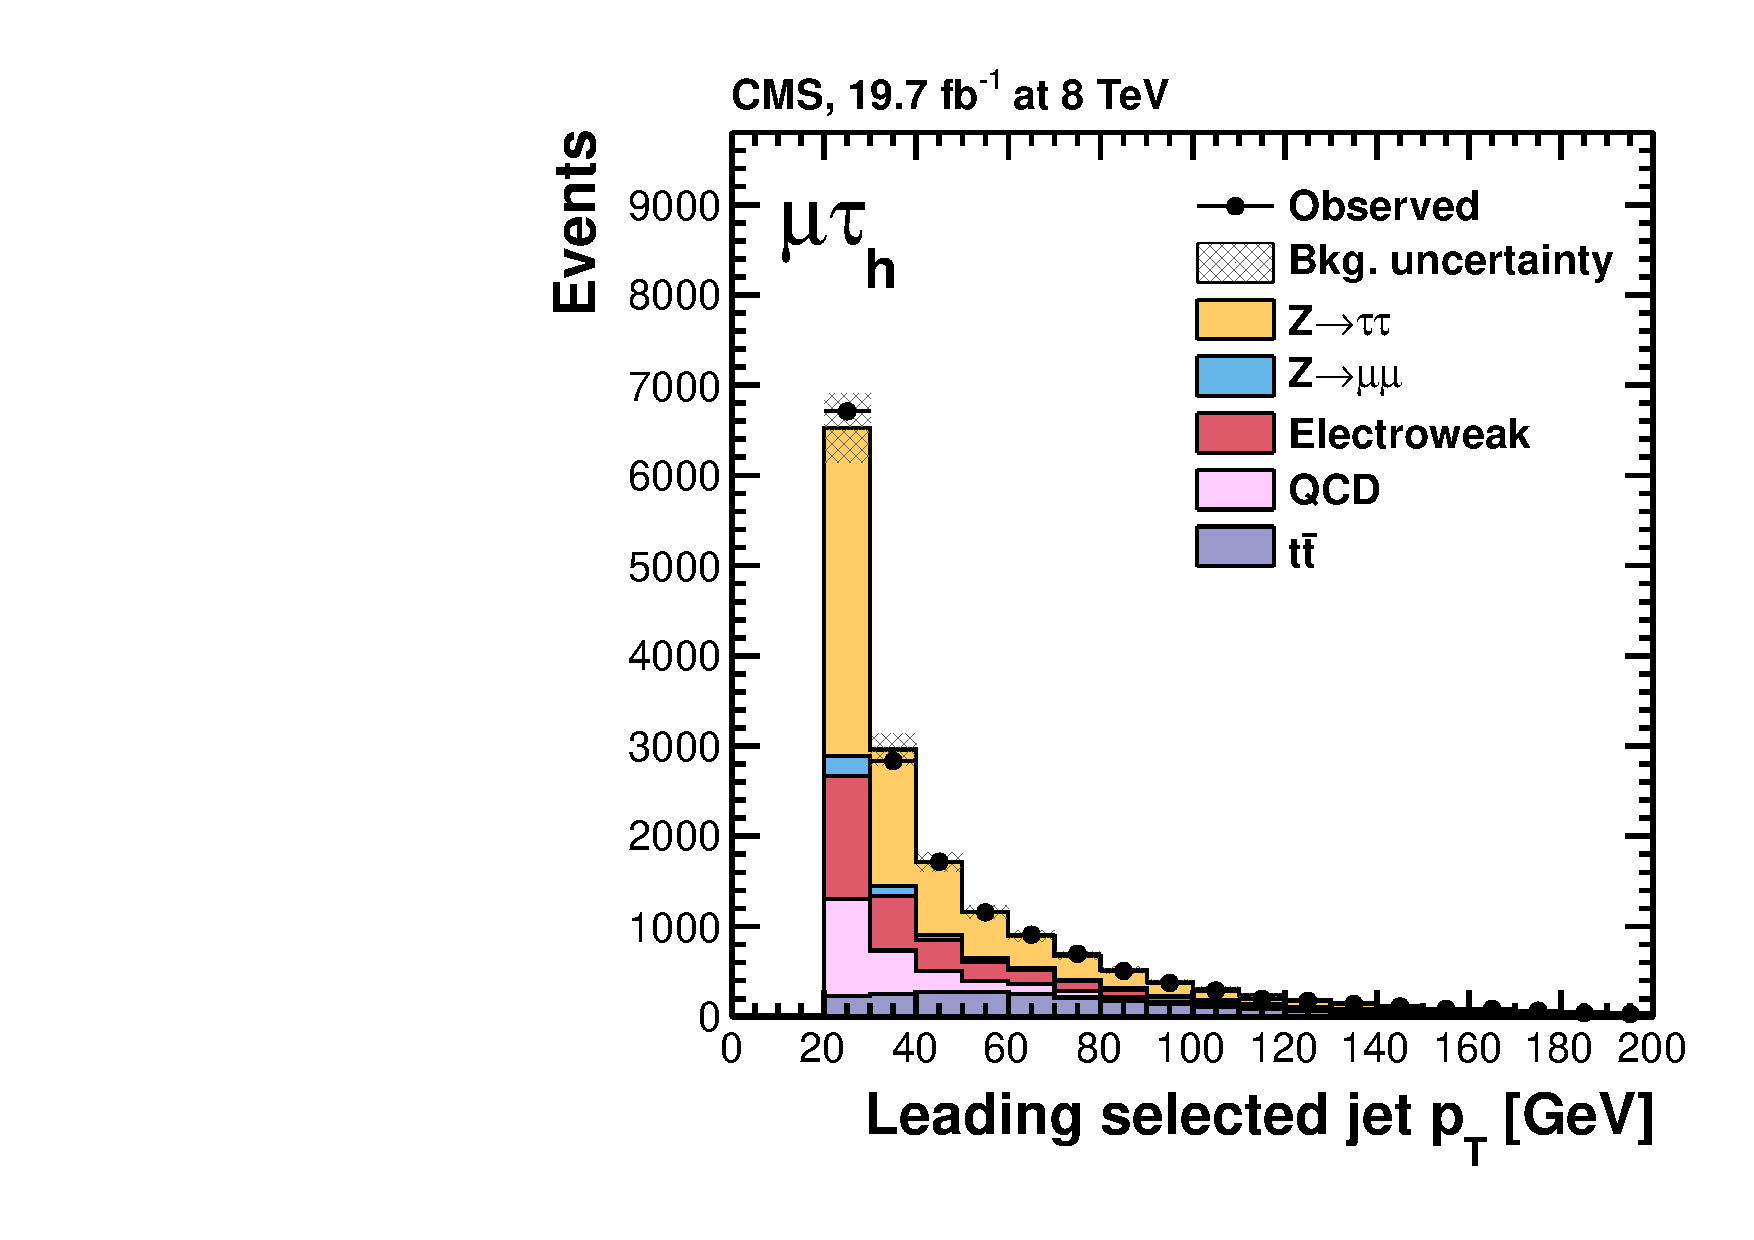
\includegraphics[width=0.4\textwidth]
      {plots/Hhh/ControlPlots/mutau/prebjetpt_1_2jetinclusive_mt_2012.pdf}}
\subfloat[]{
    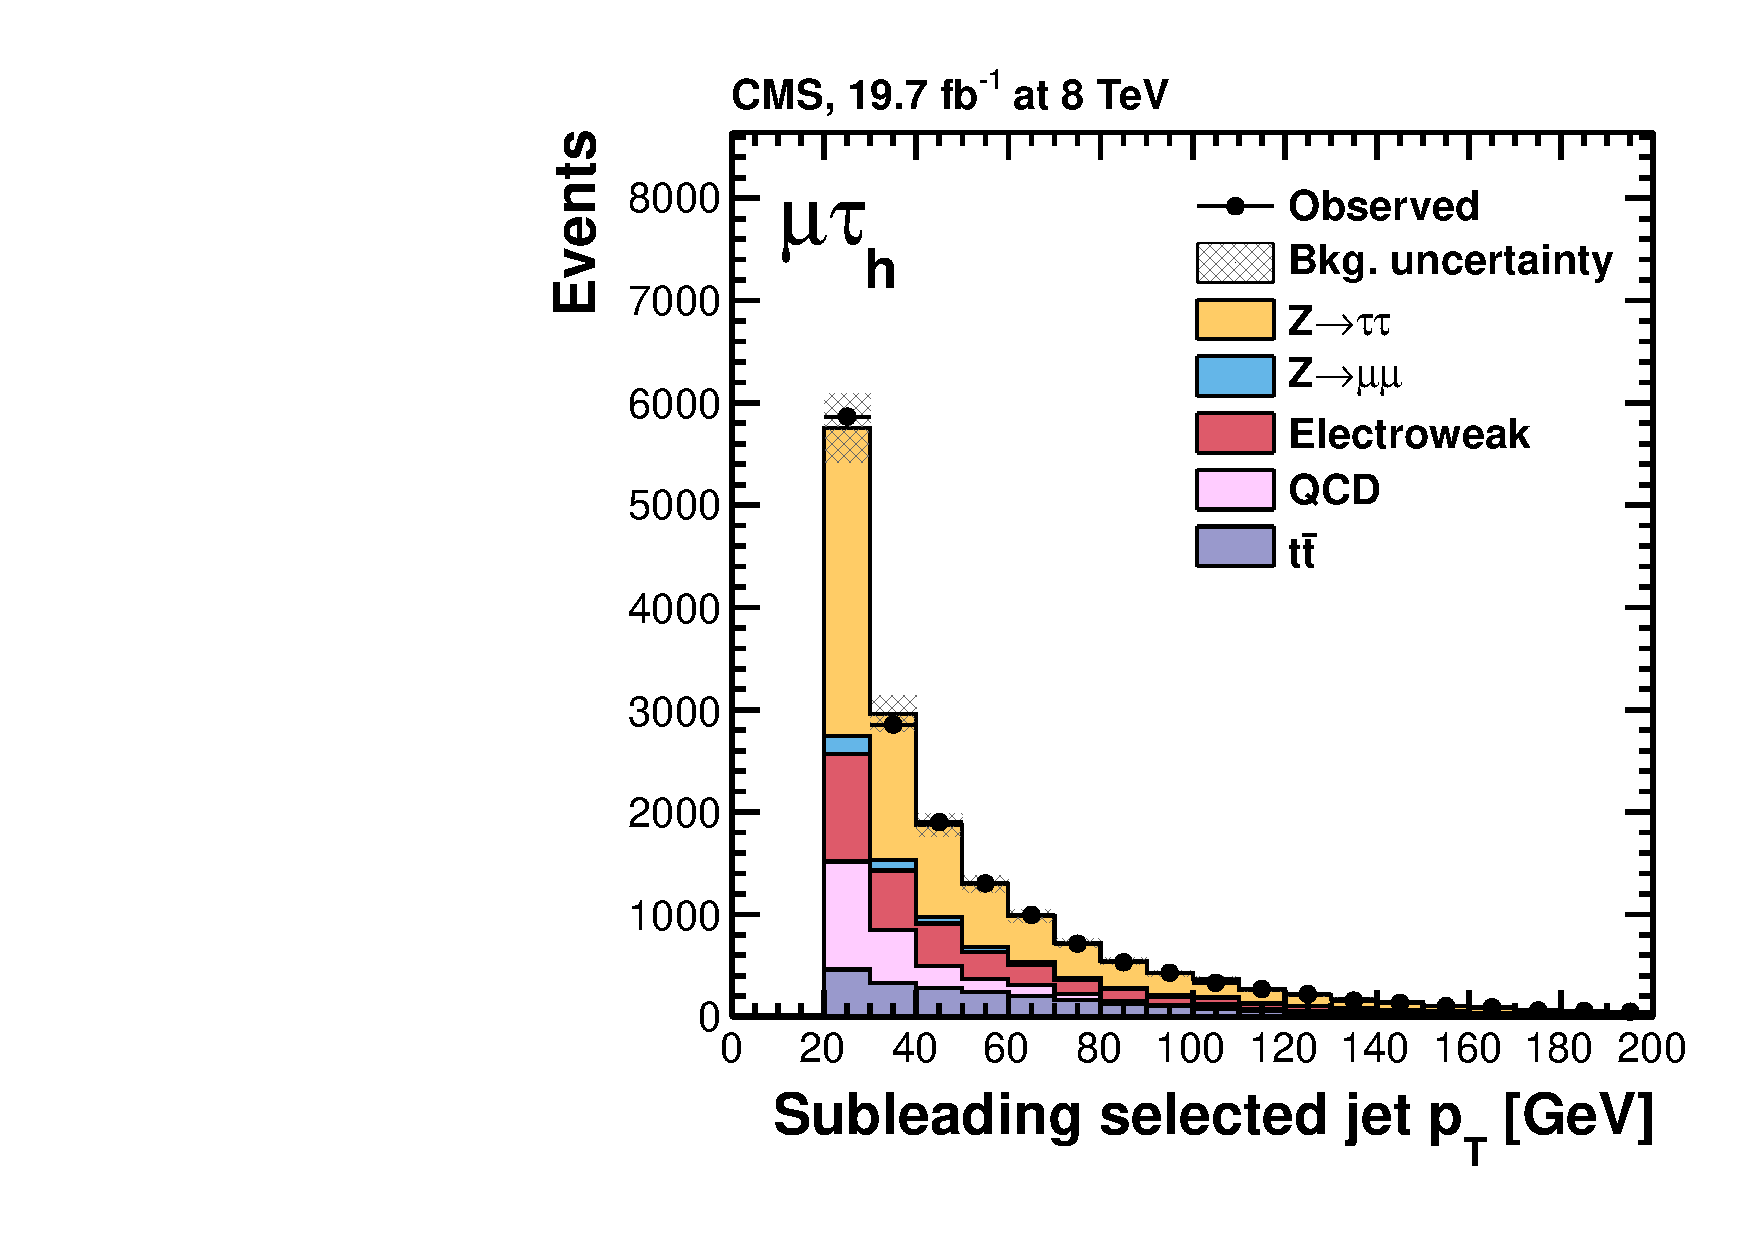
\includegraphics[width=0.4\textwidth] 
      {plots/Hhh/ControlPlots/mutau/prebjetpt_2_2jetinclusive_mt_2012.pdf}} 

\subfloat[]{
    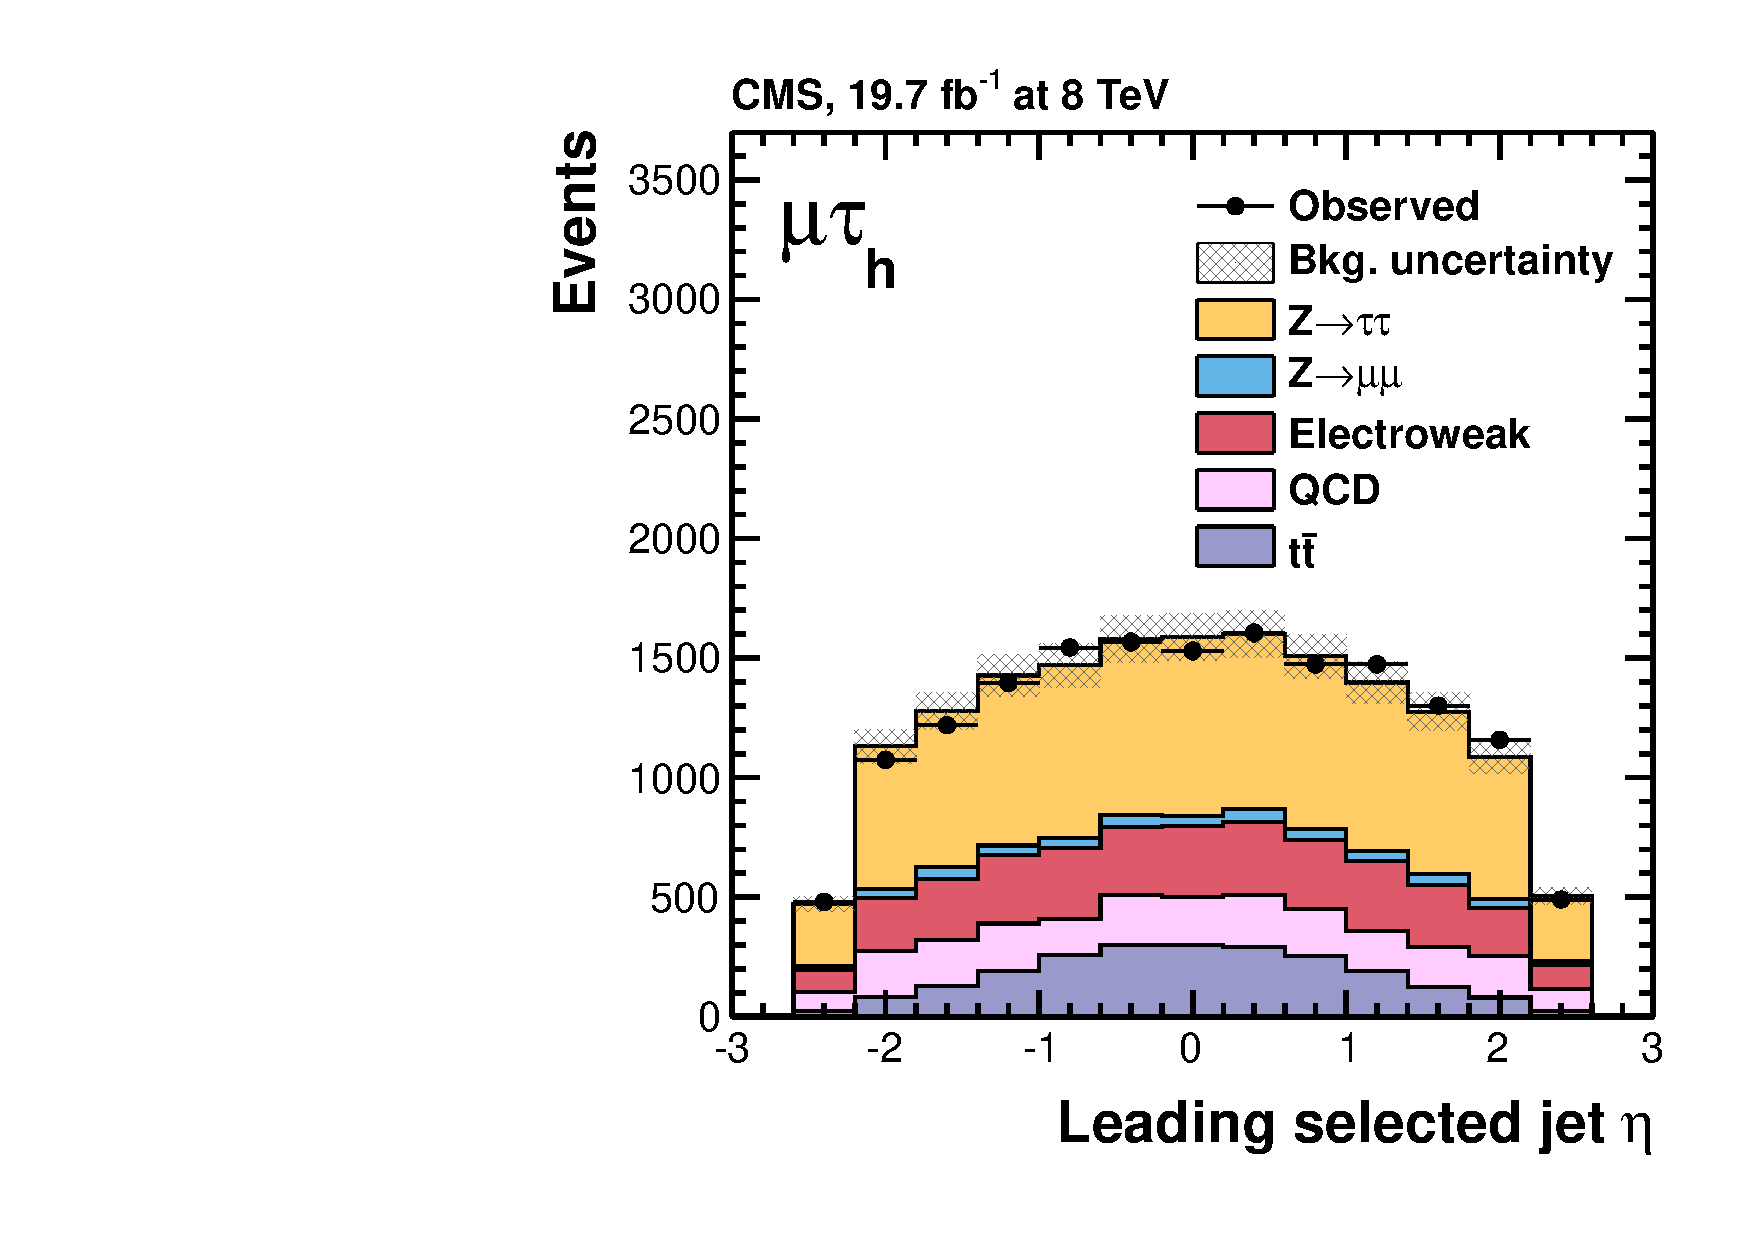
\includegraphics[width=0.4\textwidth]
      {plots/Hhh/ControlPlots/mutau/prebjeteta_1_2jetinclusive_mt_2012.pdf}}
\subfloat[]{
    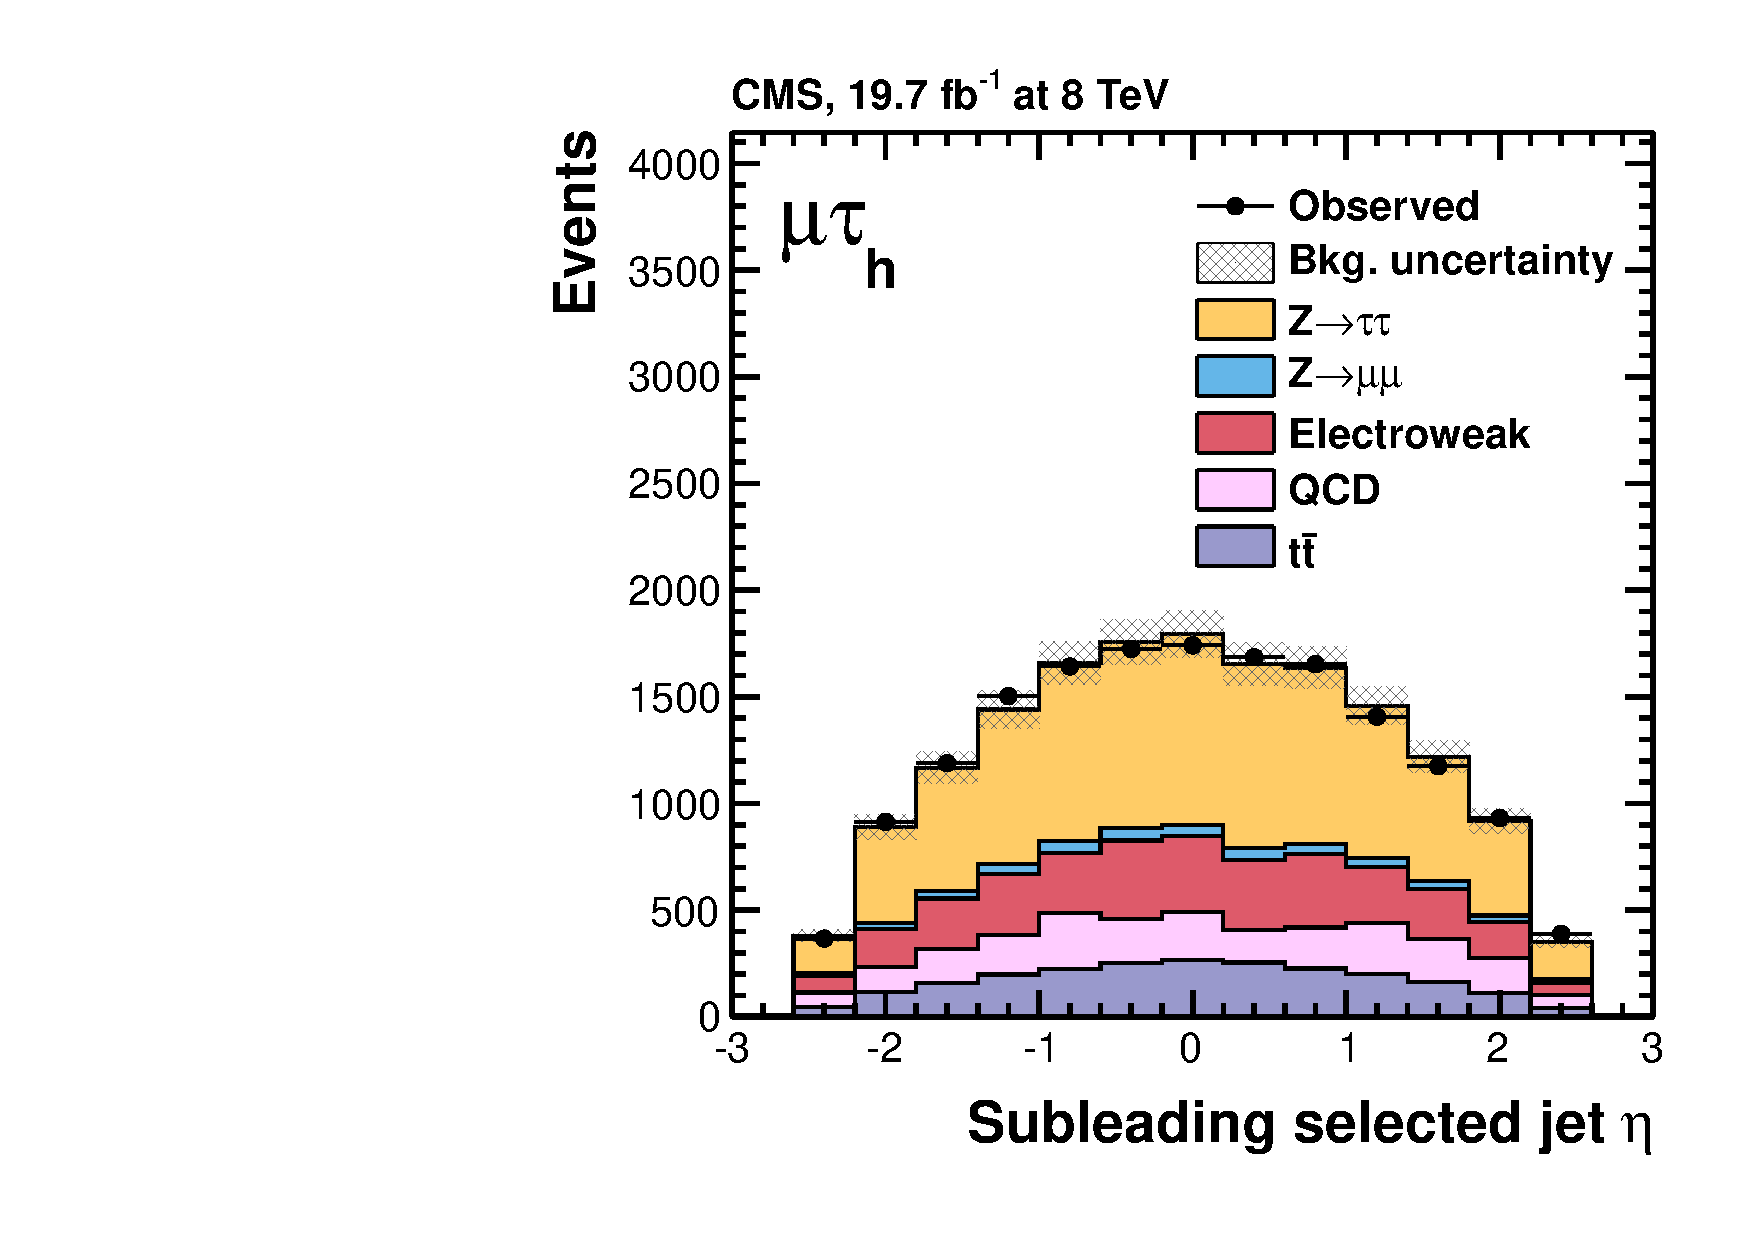
\includegraphics[width=0.4\textwidth]
      {plots/Hhh/ControlPlots/mutau/prebjeteta_2_2jetinclusive_mt_2012.pdf}} 

\subfloat[]{
    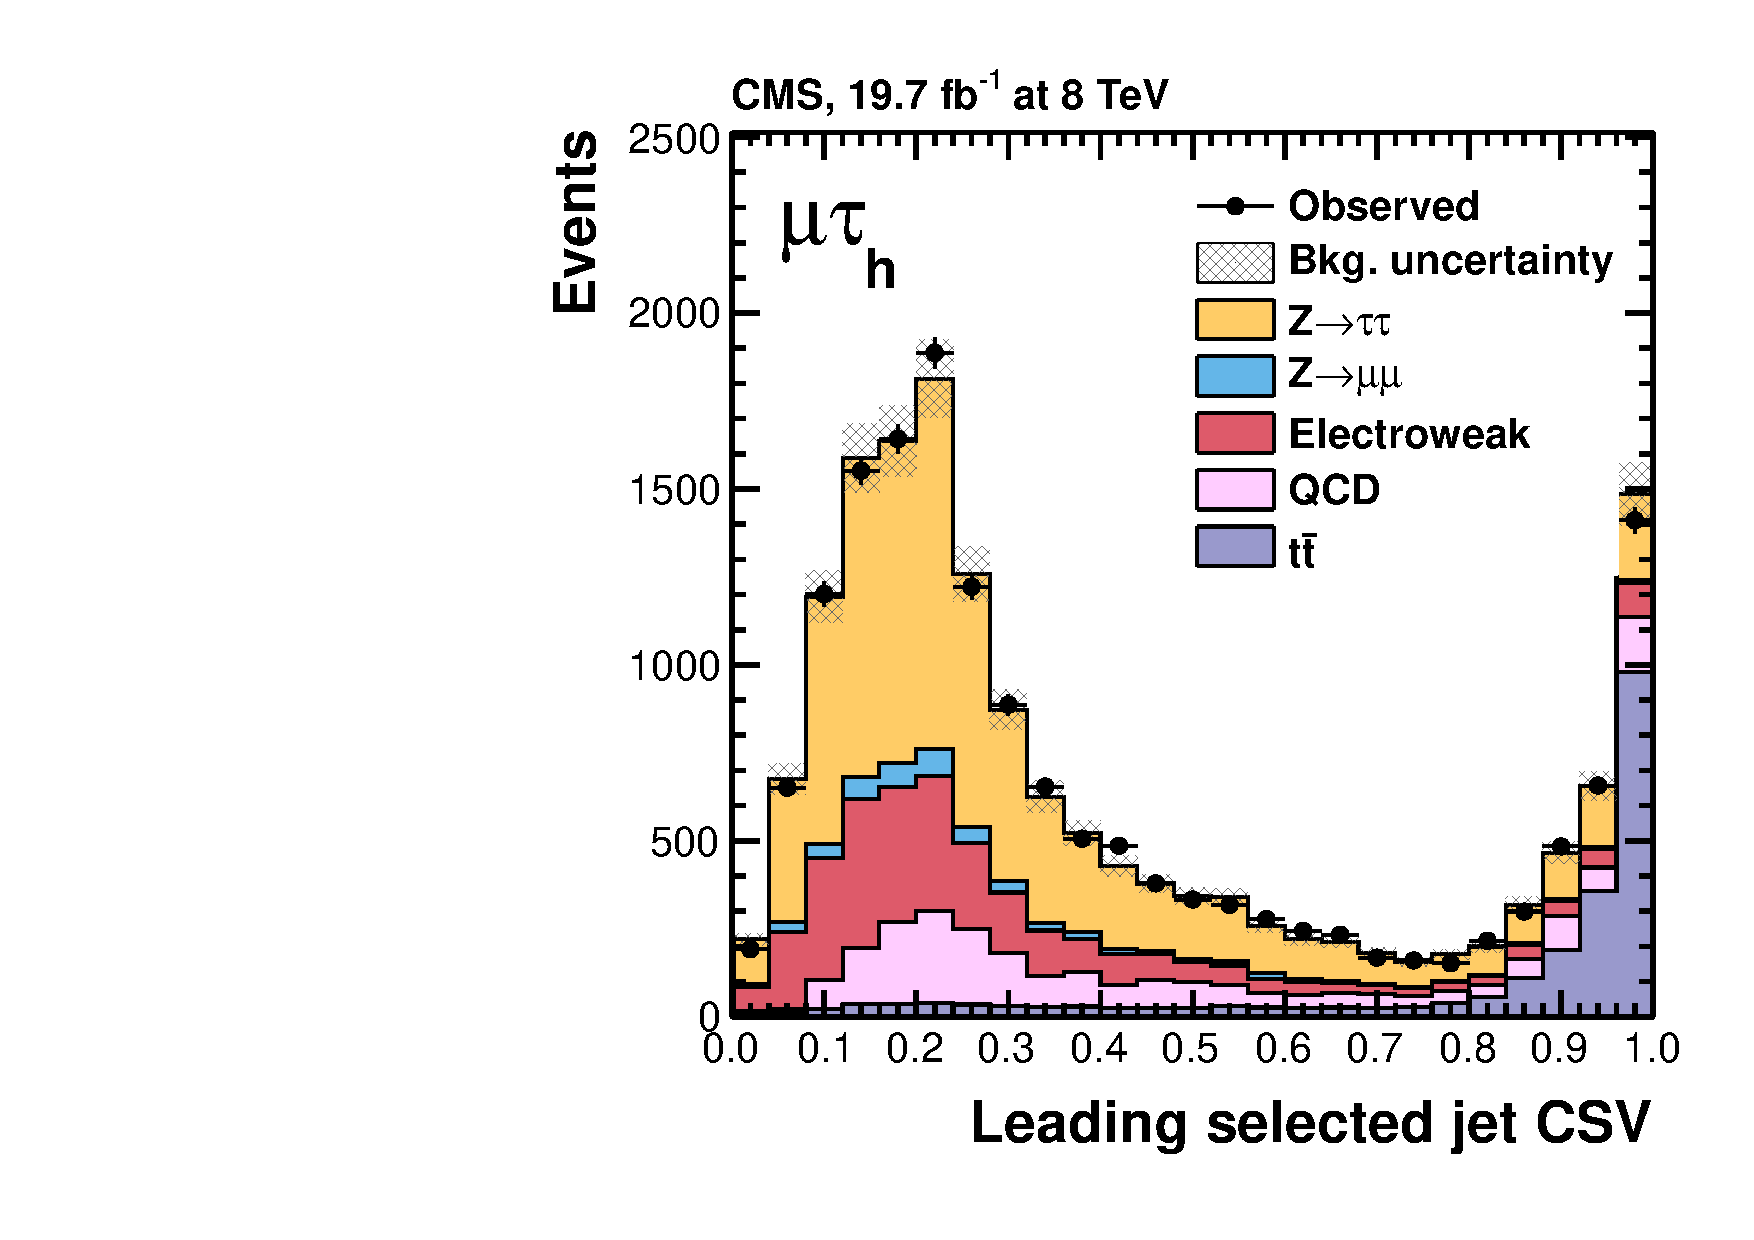
\includegraphics[width=0.4\textwidth]
      {plots/Hhh/ControlPlots/mutau/prebjetbcsv_1_2jetinclusive_mt_2012.pdf}}
\subfloat[]{
    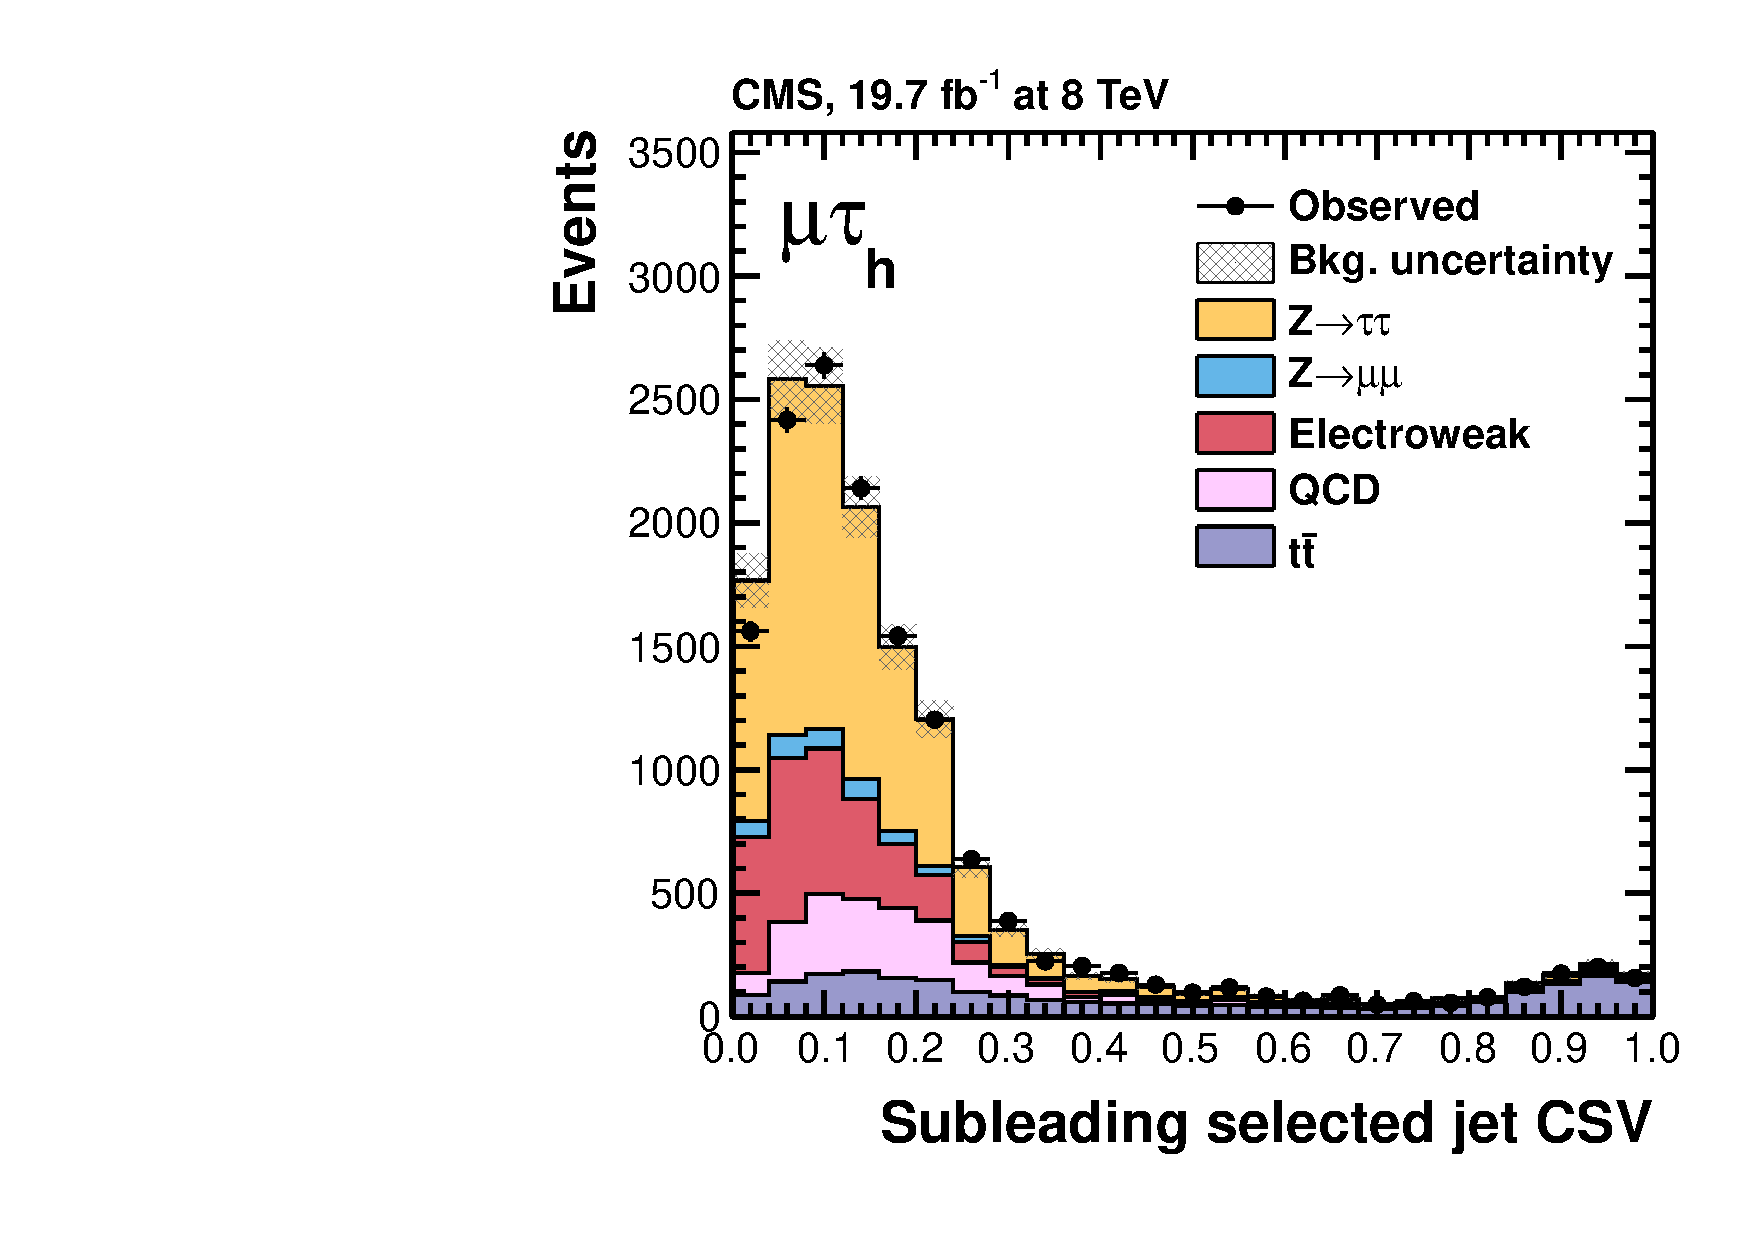
\includegraphics[width=0.4\textwidth]
      {plots/Hhh/ControlPlots/mutau/prebjetbcsv_2_2jetinclusive_mt_2012.pdf}}
\end{center}
\caption{
  Distributions of relevant kinematic variables related to the b-jet candidates for
  events with at least 2 jets in the $\mu\tau_{had}$ channel. The plots/Hhh show the
  $\pt$ (top), $\eta$ (centre) and CSV discriminator (bottom) for the leading
  jet (left) and sub-leading jet (right). Here leading and sub-leading refers to
  the jet with the highest and second highest CSV value respectively.
  Expected background contributions are shown for the values of nuisance parameters
  obtained by fitting the signal plus background hypothesis to the data.
}
\label{fig:resultsControlPlotsJetPairMuTau}
\end{figure} 

\begin{figure}
\setlength{\unitlength}{1mm}
\begin{center}
\begin{picture}(150,210)(0,0)
\put(-5.5, 140.0){\mbox{\includegraphics*[height=68mm]
  {plots/Hhh/ControlPlots/etau/mt_1_2jetinclusive_et_2012.pdf}}}
\put(78.0, 140.0){\mbox{\includegraphics*[height=68mm]
  {plots/Hhh/ControlPlots/etau/met_2jetinclusive_et_2012.pdf}}}
\put(-5.5, 70.0){\mbox{\includegraphics*[height=68mm]
  {plots/Hhh/ControlPlots/etau/pt_1_2jetinclusive_et_2012.pdf}}}
\put(78.0, 70.0){\mbox{\includegraphics*[height=68mm]
  {plots/Hhh/ControlPlots/etau/pt_2_2jetinclusive_et_2012.pdf}}}
\put(-5.5, 0.0){\mbox{\includegraphics*[height=68mm]
  {plots/Hhh/ControlPlots/etau/eta_1_2jetinclusive_et_2012.pdf}}}
\put(78.0, 0.0){\mbox{\includegraphics*[height=68mm]
  {plots/Hhh/ControlPlots/etau/eta_2_2jetinclusive_et_2012.pdf}}}
\end{picture}
\end{center}
\caption{
  Distributions of relevant kinematic variables for events with at least 2 jets
  in the $e\tau_{had}$ channel. The variable $m_{T}$ is shown in the top left
  plot and a cut of $m_{T} < 30$ is applied for the rest of the plots/Hhh, which
  show the $\MET$ (top right) $\pt$ of the electron (left centre) and tau (right
  centre), and $\eta$ of the electron (left bottom) and tau (right bottom).
  Expected background contributions are shown for the values of nuisance parameters
  obtained by fitting the signal plus background hypothesis to the data.
}
\label{fig:resultsControlPlotsTauPairETau}
\end{figure} 

\begin{figure}
\setlength{\unitlength}{1mm}
\begin{center}
\begin{picture}(150,210)(0,0)
\put(-5.5, 140.0){\mbox{\includegraphics*[height=68mm]
  {plots/Hhh/ControlPlots/etau/prebjetpt_1_2jetinclusive_et_2012.pdf}}}
\put(78.0, 140.0){\mbox{\includegraphics*[height=68mm]
  {plots/Hhh/ControlPlots/etau/prebjetpt_2_2jetinclusive_et_2012.pdf}}}
\put(-5.5, 70.0){\mbox{\includegraphics*[height=68mm]
  {plots/Hhh/ControlPlots/etau/prebjeteta_1_2jetinclusive_et_2012.pdf}}}
\put(78.0, 70.0){\mbox{\includegraphics*[height=68mm]
  {plots/Hhh/ControlPlots/etau/prebjeteta_2_2jetinclusive_et_2012.pdf}}}
\put(-5.5, 0.0){\mbox{\includegraphics*[height=68mm]
  {plots/Hhh/ControlPlots/etau/prebjetbcsv_1_2jetinclusive_et_2012.pdf}}}
\put(78.0, 0.0){\mbox{\includegraphics*[height=68mm]
  {plots/Hhh/ControlPlots/etau/prebjetbcsv_2_2jetinclusive_et_2012.pdf}}}
\end{picture}
\end{center}
\caption{
  Distributions of relevant kinematic variables related to the b-jet candidates for
  events with at least 2 jets in the $e\tau_{had}$ channel. The plots/Hhh show the
  $\pt$ (top), $\eta$ (centre) and CSV discriminator (bottom) for the leading
  jet (left) and sub-leading jet (right). Here leading and sub-leading refers to
  the jet with the highest and second highest CSV value respectively.
  Expected background contributions are shown for the values of nuisance parameters
  obtained by fitting the signal plus background hypothesis to the data.
}
\label{fig:resultsControlPlotsJetPairETau}
\end{figure} 





